\section{Descrizione del Modello}
Il modello considerato \cite{mostafizi2019agent} é un sistema multi-agente che prevede l'evacuazione della città di Seaside, Oregon in caso di tsunami di auto e pedoni.
%
% TODO: riscrivere
L'evacuazione non include le conseguenze del terremoto che avviene prima dello tsunami e viene considerata iniziare alla fine di questo.
Il modello è basato sull'uso di dati GIS per la distribuzione della popolazione, la rete stradale ed i rifugi.

%
Per la distribuzione della popolazione é stato considerato uno scenario a mezzogiorno di un fine settimana di estate,
che presenta una maggiore concentrazione di residenti sulla spiaggia e nel centro della città
La popolazione sulla costa e nel centro é distribuita normalmente,
mentre quella nella zona residenziale é distribuita uniformemente (Fig. \ref{fig:population}).

\begin{figure}[ht]
  \centering
  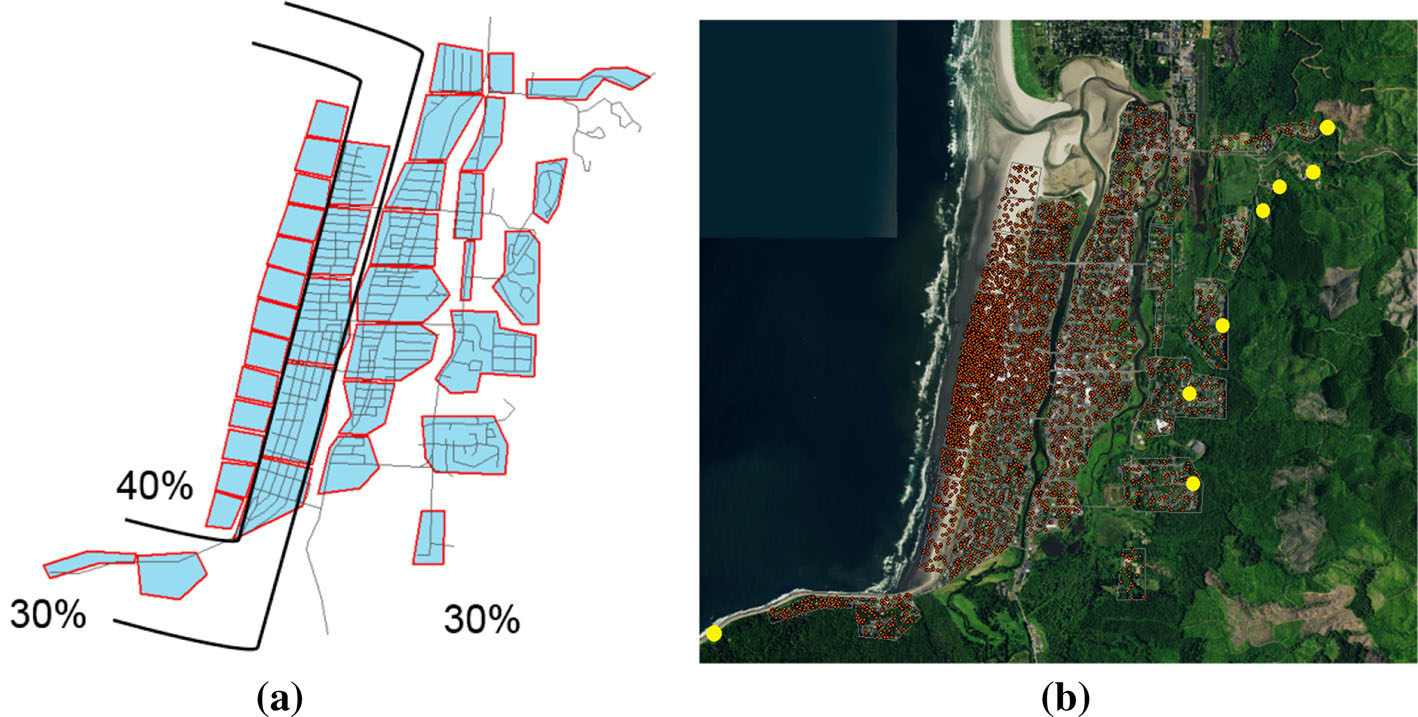
\includegraphics[width=0.82\textwidth]{images/population}
  \caption{Distribuzione della popolazione nello scenario considerato.
    (a) Mostra le aree in cui è distribuita la popolazione, divise nelle tre macro aree: costa, centro, zona residenziale.
    (b) Immagine satellitare con la distribuzione della popolazione.}
  \label{fig:population}
\end{figure}

\subsection{Ambiente}
L'ambiente é composto dalla rete stradale della città con i relativi rifugi e dello tsunami.

% TODO: riscrivere
La rete stradale é rappresentata da un grafo, i cui nodi corrispondono alle intersezioni e gli archi alle strade.
Tutte le strade sono considerate a senso unico, con una sola corsia e con una velocità limite di 55 km/h.

8 delle intersezioni sono marcate come rifugi con capacità illimitata.

Lo tsunami é rappresentato da una griglia discreta, dove ogni cella contiene i valori temporali di altezza delle onde.
I dati usati in questo progetto sono quelli calcolati dal modello di inondazione ComMIT/MOST \cite{titov1997implementation} per la zona di subduzione della Cascadia.


\subsection{Agenti}
La simulazione può prevedere diversi tipi di agenti: residenti, pedoni e auto.

\subsubsection{Residenti}
All'inizio dell'evacuazione i residenti si trovano all'esterno di edifici e auto
e autonomamente scelgono come evacuare. % TODO: mmmmh
Un residente può scegliere diverse modalità per evacuare: a piedi o in auto e raggiungere un rifugio verticale oppure orizzontale.
Una volta che ogni agente decide in che modo evacuare non cambierà scelta per tutta la simulazione.

\vspace*{4mm}
Il tempo impiegato per prepararsi all'evacuazione (milling time) é modellato tramite
la distribuzione di Rayleigh (Eq. \ref{eq:rayleigh}), con un tempo minimo ($\tau$) di 10 minuti
e un parametro di scala ($\sigma$) di 1.65.
Questo tempo comprende anche il raggiungimento del veicolo.

\begin{equation}
  f(x; \tau, \sigma) = \frac{(x - \tau)^2}{\sigma^2}e^{-{(x - \tau)^2}/(2\sigma^2)}
  \label{eq:rayleigh}
\end{equation}

Scaduto il tempo di preparazione l'agente si muove verso l'intersezione più vicina e
in base alla modalità scelta viene considerato un agente di tipo pedone o auto.
L'agente quindi inizia a seguire il percorso più breve per il rifugio più vicino raggiungibile, trovato tramite l'algoritmo A*.

Gli agenti durante l'evacuazione possono continuare sulla strada attuale o cambiare strada seguendo il percorso,
morire se l'altezza dell'onda nel punto in cui si trova é superiore o uguale a un parametro $H_c$,

\subsubsection{Pedoni}
La velocità di camminata viene stabilita tramite una distribuzione normale
con media 1.21 m/s e deviazione standard 0.20 m/s.
La velocità di ogni pedone rimane costante durante tutta l'evacuazione.

% Non viene gestita alcuna interazione Pedone-Pedone o Pedone-Auto.

\newpage
\subsubsection{Auto}
Ogni auto conteniene una sola persona per considerare il caso peggiore.
Le auto possono raggiungere la velocità massima imposta dalla strada, ovvero 55 km/h.

Il comportamento delle auto é modellato tramite il modello car-following, General-Motors.

La teoria sui modelli Car following descrivono come un veicolo ne segue un'altro
e cambi il proprio comportamenteo reagendo a quest'ultimo.

\begin{figure}[ht]
  \centering
  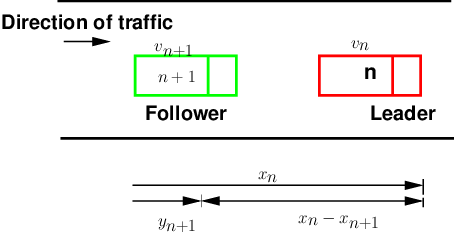
\includegraphics[width=0.9\textwidth]{images/GM.png}
  \label{fig:general-motors-img}
  \caption{schema generale dei modelli car following, dove n+1 è il veicolo corrente ed n quello di fronte, $v_{n+1}, v_{n}$ sono le rispetive velocità, mentre $x_{n+1}, x_{n}$ sono le rispettive posizioni è $x_{n} - x_{n + 1}$ è la distanza tra i due veicoli.}
\end{figure}

Secondo il modello General-Motors ogni auto risponde alle condizioni del traffico circostante esclusivamente accellerando o decelerando, l'accellerazione dipende dalla velocità del veicolo corrente, la sua posizione relativa e la velocità con il veicolo di fronte.
Basato sul concetto follow-the leader fondato su due assunzioni principali:
più veloce è il veicolo di fronte maggiore sarà la distanza tra i due veicoli,
inoltre una certa distanza di sicurezza dall'auto in fronte deve essere mantenuta.

\begin{equation}
  a_{n+1}^{t} = [ \frac{\alpha_{l, m} * (v_{n + 1}^{t})^{m} }{ (x_{n}^{t} - x_{n + 1}^{t})^{l}}][v_{n}^{t} - v_{n + 1}^{t}]
  \label{eq:general-motors-eq}
\end{equation}

\noindent
Equation 2: qui viene riportata l'equazione principale del modello General-Motors, 
dove l è un esponente di distanza con il veicolo di fronte che può assumere valori da +4 a -1,
m è un esponente di velocità con valori tra -2 a +2, $\alpha$ è un coefficiente di sensitività.






\section{Estensione del Modello}
Il modello é stato esteso andando a gestire le interazioni tra gli agenti nelle intersezioni.

\subsection{Comportamento dei Pedoni}
E' stata aggiunta una variabilità nella velocità di camminata

Marciapiedi
Striscie pedonali

\subsection{Gestione degli Intersezioni}
